\usetikzlibrary{positioning}
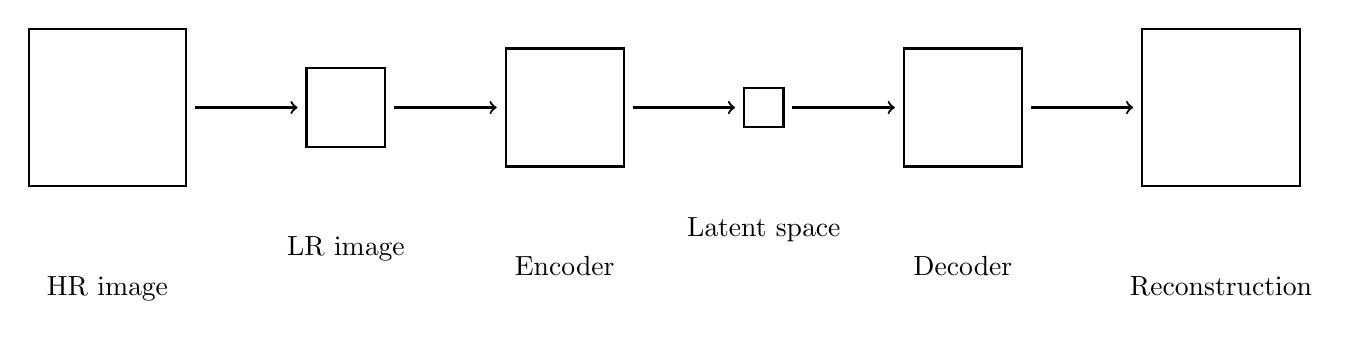
\begin{tikzpicture}[x = 1cm, y = 1cm, thick,
		image/.style={rectangle, draw, inner sep = 0pt, minimum size = 2 cm},
		network/.style={rectangle, draw, inner sep = 0pt, minimum size = 2 cm},
		arrow/.style={ ->, shorten <= 1 mm, shorten >= 1 mm}
	]
	
	\node[image, minimum size = 2 cm] (HR) at (0, 0) {};
	\node[below = of HR] {HR image};
	
	\node[image, minimum size = 1 cm, right = 1.5 cm of HR] (LR) {};
	\node[below = of LR] {LR image};
	
	\node[network, minimum size = 1.5 cm, right = 1.5 cm of LR] (encoder) {};
	\node[below = of encoder] {Encoder};
	
	\node[network, minimum size = 0.5 cm, right = 1.5 cm of encoder] (latent) {};
	\node[below = of latent] {Latent space};
	
	\node[network, minimum size = 1.5 cm, right = 1.5 cm of latent] (decoder) {};
	\node[below = of decoder] {Decoder};
	
	\node[image, minimum size = 2 cm, right = 1.5 cm of decoder] (reconstruction) {};
	\node[below = of reconstruction] {Reconstruction};
	
	\draw[arrow] (HR) -- (LR);
	\draw[arrow] (LR) -- (encoder);
	\draw[arrow] (encoder) -- (latent);
	\draw[arrow] (latent) -- (decoder);
	\draw[arrow] (decoder) -- (reconstruction);
	
\end{tikzpicture}
